\section{高效邻域粒子查找算法}
    SPH方法以粒子作为采样点来离散采样空间中的物理量,如速度、密度、压强、作用力等等。这些物理量又需要其他粒子通过核函数加权求和来确定。而核函数是紧支撑的,所以在计算是仅需要确定每个粒子周围的邻域粒子集合即可,这是SPH流体模拟中非常重要的一个步骤,它的准确性和效率直接影响到SPH的仿真稳定性,计算精度和速度。
    
    \begin{figure}[htbp]
    	\centering
    	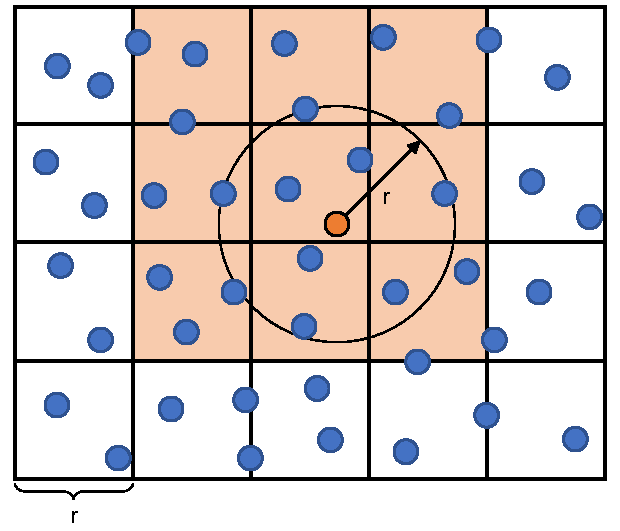
\includegraphics[width=.35\textwidth]{figures/neighbor/uniform_grid.pdf}
    	\caption{均匀网格划分}
    \end{figure}

\subsection{方法概述}
    查找邻域粒子的过程可以分为两个阶段,第一阶段是对每个粒子构建邻域粒子索引集合,第二阶段是在计算物理量时直接通过这个集合查找邻域粒子。查找阶段的时间复杂度是 $O(mn)$,$m$ 为邻域粒子的最大数量,在具体实现时是一个确定的常数,所以查找阶段可以达到线性复杂度 $O(n)$。而对于索引集合的构建,穷举算法的时间复杂度是 $O(n^2)$,SPH模拟中仿真粒子的数量非常大,这样做的性能开销是往往不可接受的,所以这个阶段是算法优化的重点。
    
    优化算法的基本思路是,将空间划分为均匀网格,找到每个网格中包含的所有粒子,然后在确定邻域粒子集合时,只需要计算周围网格中包含的粒子即可。如果网格中粒子最大数量为 $k$,则优化算法的时间复杂度为 $O(kn)$。
    
    具体来说,如果核函数半径为 $r$(即邻域搜索半径为 $r$),可以将空间划分为间距为 $r$ 的网格。在计算粒子 $p$ 的邻域粒子集合时,仅需要查找 $p$ 所在网格与相邻网格中的粒子,在三维空间中共27个网格。算法实现共分为两个步骤,空间网格划分和构建邻域粒子集合。这两个步骤所涉及的数据结构在逻辑上可以抽象为一种,将下一节详细介绍。

    \begin{figure}
    	\centering
    	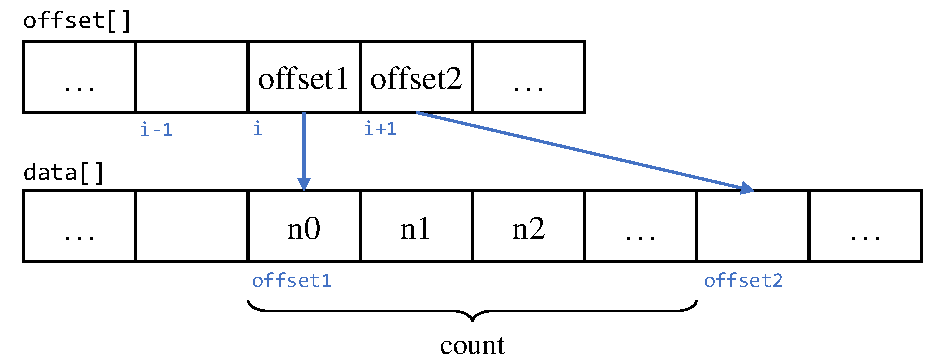
\includegraphics[width=.55\textwidth]{figures/neighbor/data_structure.pdf}
    	\caption{集合数组数据结构}
    \end{figure}

    \begin{table}
	\centering
	\caption{集合数组存储格式对比}
	\begin{tabular}{lll}
	\toprule
	数据结构 & 优点 & 缺点 \\
	\midrule
	\multirow{2}{*}{定长格式}
	& 1. 实现简单。  & 1. 存储空间消耗大。  \\
	& 2. 支持随机存取。  & 2. 存储碎片化,读取效率较低。  \\
	\hline
	\multirow{3}{*}{不定长格式} 
	& 1. 支持随机存取。  & 1. 实现较复杂。 \\
	& 2. 存储空间无额外消耗。  & 2. 写入时需要额外的计算步骤。  \\
	& 3. 存储连续,读取效率高。  &   \\
	\bottomrule
	\end{tabular}
\end{table}

\subsection{集合数组}
\subsubsection{数据结构}
    邻域粒子集合和空间网格划分集合的存储数据具有一定相似结构,它们都需要存储确定数量个集合,但每个集合的元素数量不定,我们将这种抽象结构定义为集合数组。具体来说,对于邻域粒子集,粒子数量是确定的,但每个粒子邻域中的粒子数量不定。对于空间网格划分集,均匀划分后网格数量是确定的,但每个网格中粒子数量不定。如果是CPU实现,可以考虑邻接表等高级数据结构,但是对于GPU程序,需要考虑存储空间排布、并行随机读写效率等问题。这种数据结构的实现有两种格式,定长格式和不定长格式。
    
    定长格式确定了集合元素的数量上限,对于每个集合所消耗的存储空间相同。其优点为实现简单,支持随机读写。缺点为存储空间消耗较大,需要预设一个集合数量;并且存储碎片化严重,空间局部性差,难以充分利用硬件性能。
    
    不定长格式与此相反,长度不定的集合之间连续存储,可以降低存储消耗,无存储碎片。但缺点为实现较复杂,需要offset[]额外数组辅助来支持并行随机读取,在并行构建时也需要先行确定这两个数组中的数据,再写入数据。
    
    不定长格式的数据结构在存储开销的优势使得其更适合浏览器环境的流体模拟。虽然其构建开销较高,但是实际实现中数据读取次数远大于构建次数,这使得其读取效率方面的优势更为重要。

    \begin{figure}[htbp]
    	\centering
    	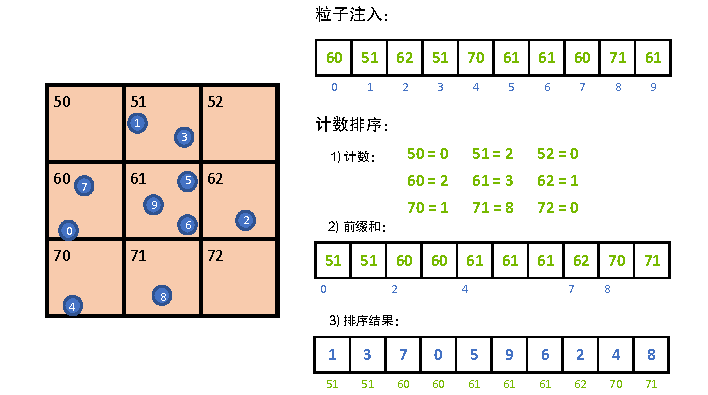
\includegraphics[width=.8\textwidth]{figures/neighbor/counting_sort.pdf}
    	\caption{计数排序}
    \end{figure}

\subsubsection{构建算法}
    最终算法实现的重要步骤就在于这两个集合数组的构建。构建邻域粒子集较简单,可以以集合为单位分配线程,在每个线程中串行地依次确定集合元素。而构建空间网格划分集较复杂,需要以集合元素为单位分配线程,在每个线程中只能确定该元素属于哪个集合,线程间还存在依赖关系。参考\cite{G10NS}和\cite{RC14NS}的方案,我们使用计数排序来确定最终结果。
    
    最终邻域粒子查找算法的计算管线为:

    \begin{enumerate}
    	\item 粒子注入,计算粒子所属网格以及网格粒子数。
    	\item 计算网格粒子数的前缀和。
    	\item 计数排序,得到空间网格划分集和。
    	\item 计算邻域粒子数量。
    	\item 计算邻域粒子数量的前缀和。
    	\item 得到邻域粒子集合。
    \end{enumerate}

    管线中2,5步骤需要计算数组前缀和,这部分将在下一节详细介绍。其他步骤并行度均等同于粒子数量,全部使用WebGPU计算管线实现。

    \begin{figure}
    	\centering
    	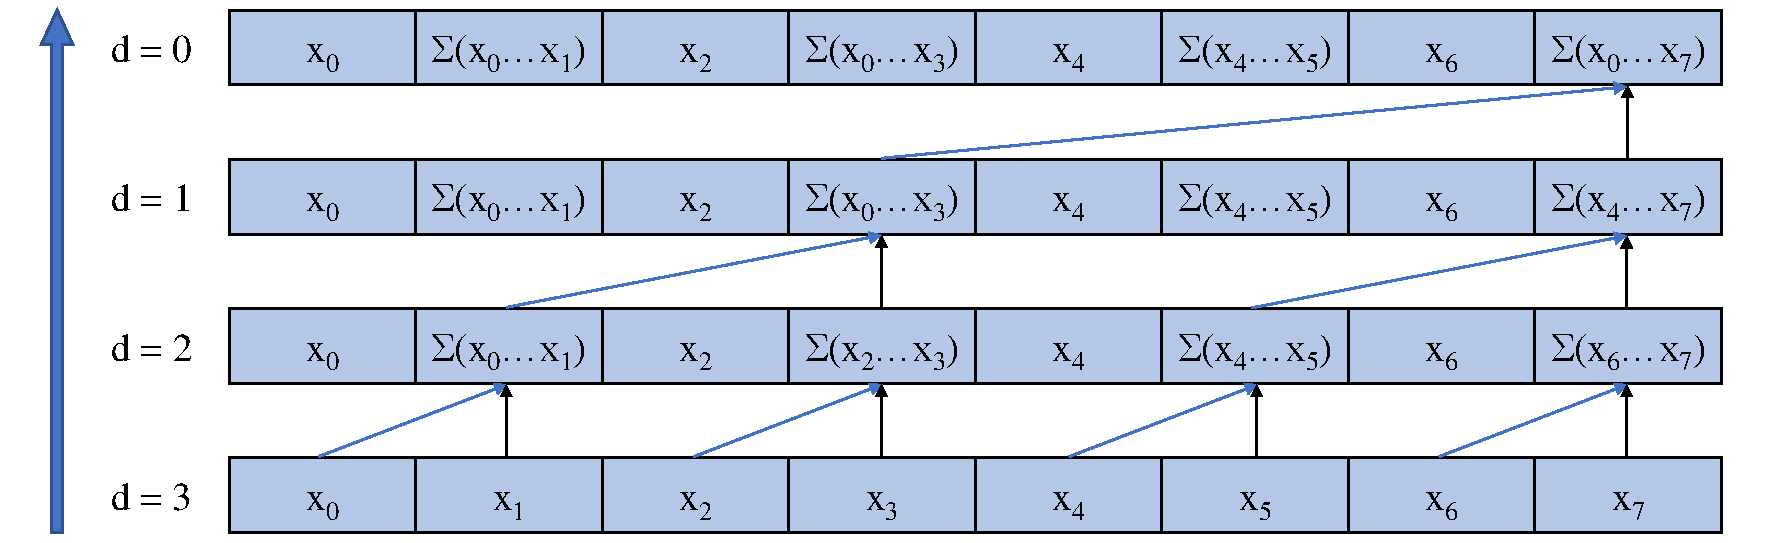
\includegraphics[width=.8\textwidth]{figures/neighbor/up_sweep.pdf}
    	\caption{自底向上扫描}
    	\label{fig:upsweep}
    \end{figure}
    
    \begin{figure}
    	\centering
    	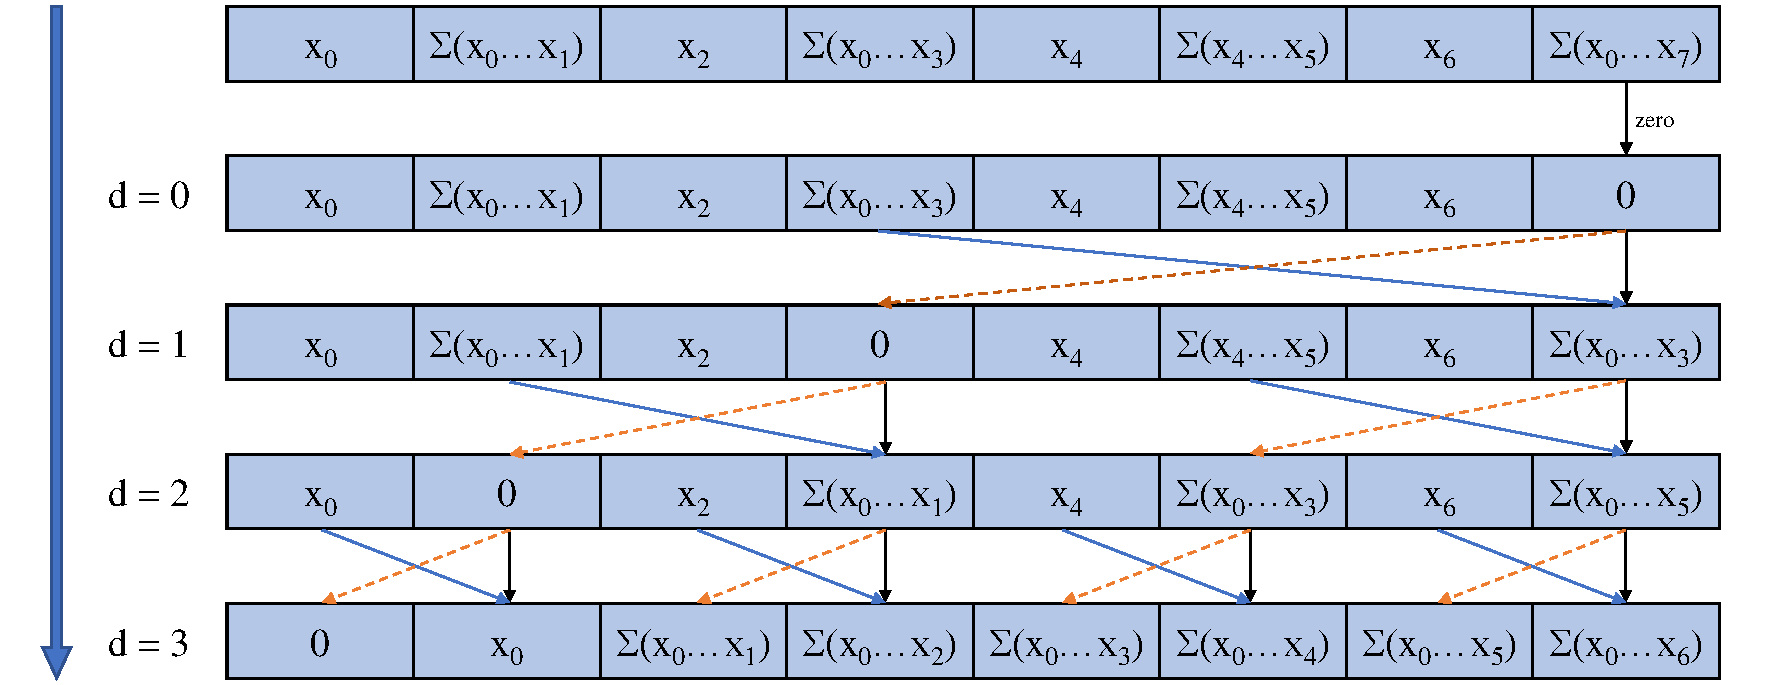
\includegraphics[width=.8\textwidth]{figures/neighbor/down_sweep.pdf}
    	\caption{自顶向下扫描}
    	\label{fig:downsweep}
    \end{figure}

\subsection{并行计算前缀和}
    对数组计算前缀和,如果是CPU串行执行,这一算法非常简单,只需要遍历一次数组即可。但是如果使用GPU并行计算大数组前缀和,就需要重新设计算法并依据硬件架构作出相应优化,才能发挥出GPU强大的并行计算能力。本文实现的前缀和算法主要参考了英伟达在CUDA上的实现\cite{HSO07SCAN} ,同时根据WebGPU的诸多限制与邻域粒子查找这一确定的应用场景,对原算法做出了相应的简化与调整。
    
    算法的基本思路为:在输入数据上建立一个平衡的二叉树(将输入数据视作二叉树叶子节点),先自底向上再自顶向下扫描两遍二叉树节点来计算前缀和。如果一个二叉树有 $n$ 个叶子节点,则树的深度为 $\log n$,每层有 $2^n$ 个节点,所以遍历一遍二叉树的计算复杂度为 $O(n)$。需要强调的是,二叉树只是算法的逻辑结构,在实际实现中并不需要构建复杂的数据结构,也不需要额外的空间存储二叉树内部节点的值。
    
    在自底向上扫描(如图\ref{fig:upsweep})阶段,每个中间节点只保存数组的部分前缀和,即此中间节点对应的叶子节点之和。
    
    在自顶向下扫描(如图\ref{fig:downsweep})阶段,每个中间节点可以根据父结点和兄弟节点的值得到完整前缀和。

    \begin{figure}
    	\centering
    	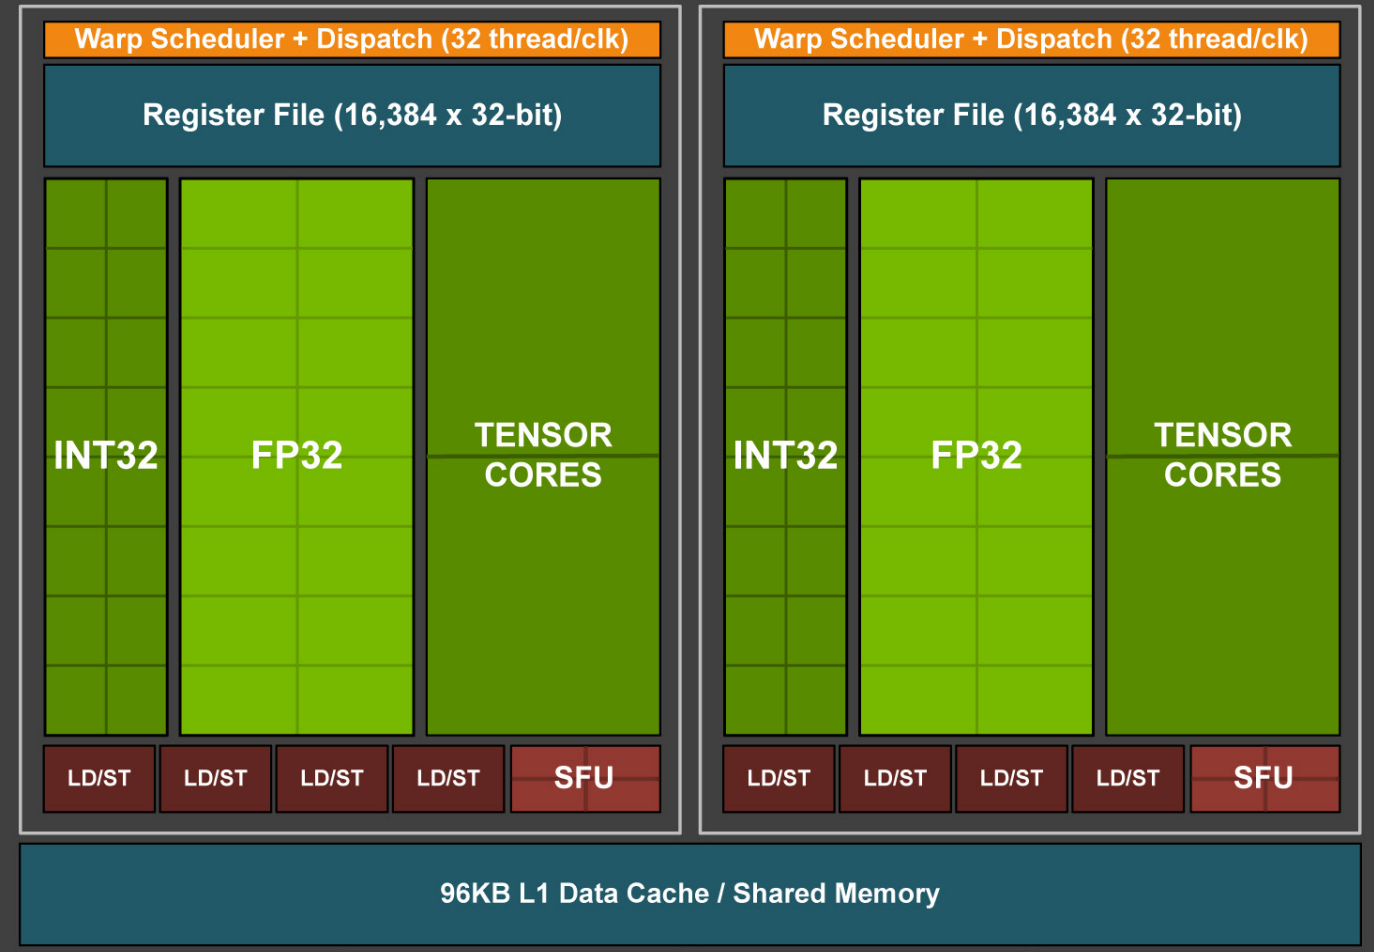
\includegraphics[width=.6\textwidth]{figures/neighbor/sm_cut.png}
    	\caption{NIVIDA Turing GPU 架构\cite{NV18Truing}}
    	\label{fig:turing}
    \end{figure}

\subsubsection{访存优化}
    GPU的存储结构(如图\ref{fig:turing})和CPU类似,同样有多级存储机制,数据主要存储在显存中,读写显存都需要花费大量时钟周期。而缓存的读写速度就会远远快于显存。GPU具有大量计算单元,称为流处理器(Stream Processor, SP),多个流处理器组成一个流多处理器(Stream Multiprocessor, SM)。一个SM有一块缓存,为SM内所有流处理器共享,称为共享内存(Shared Memory)。一般一个SM对应一个计算着色器的线程组,所以可以在一个线程组中将所有数据先载入共享内存,再完成前缀和计算,最后将共享缓冲区的计算结果写回显存。

    \begin{figure}
    	\centering
    	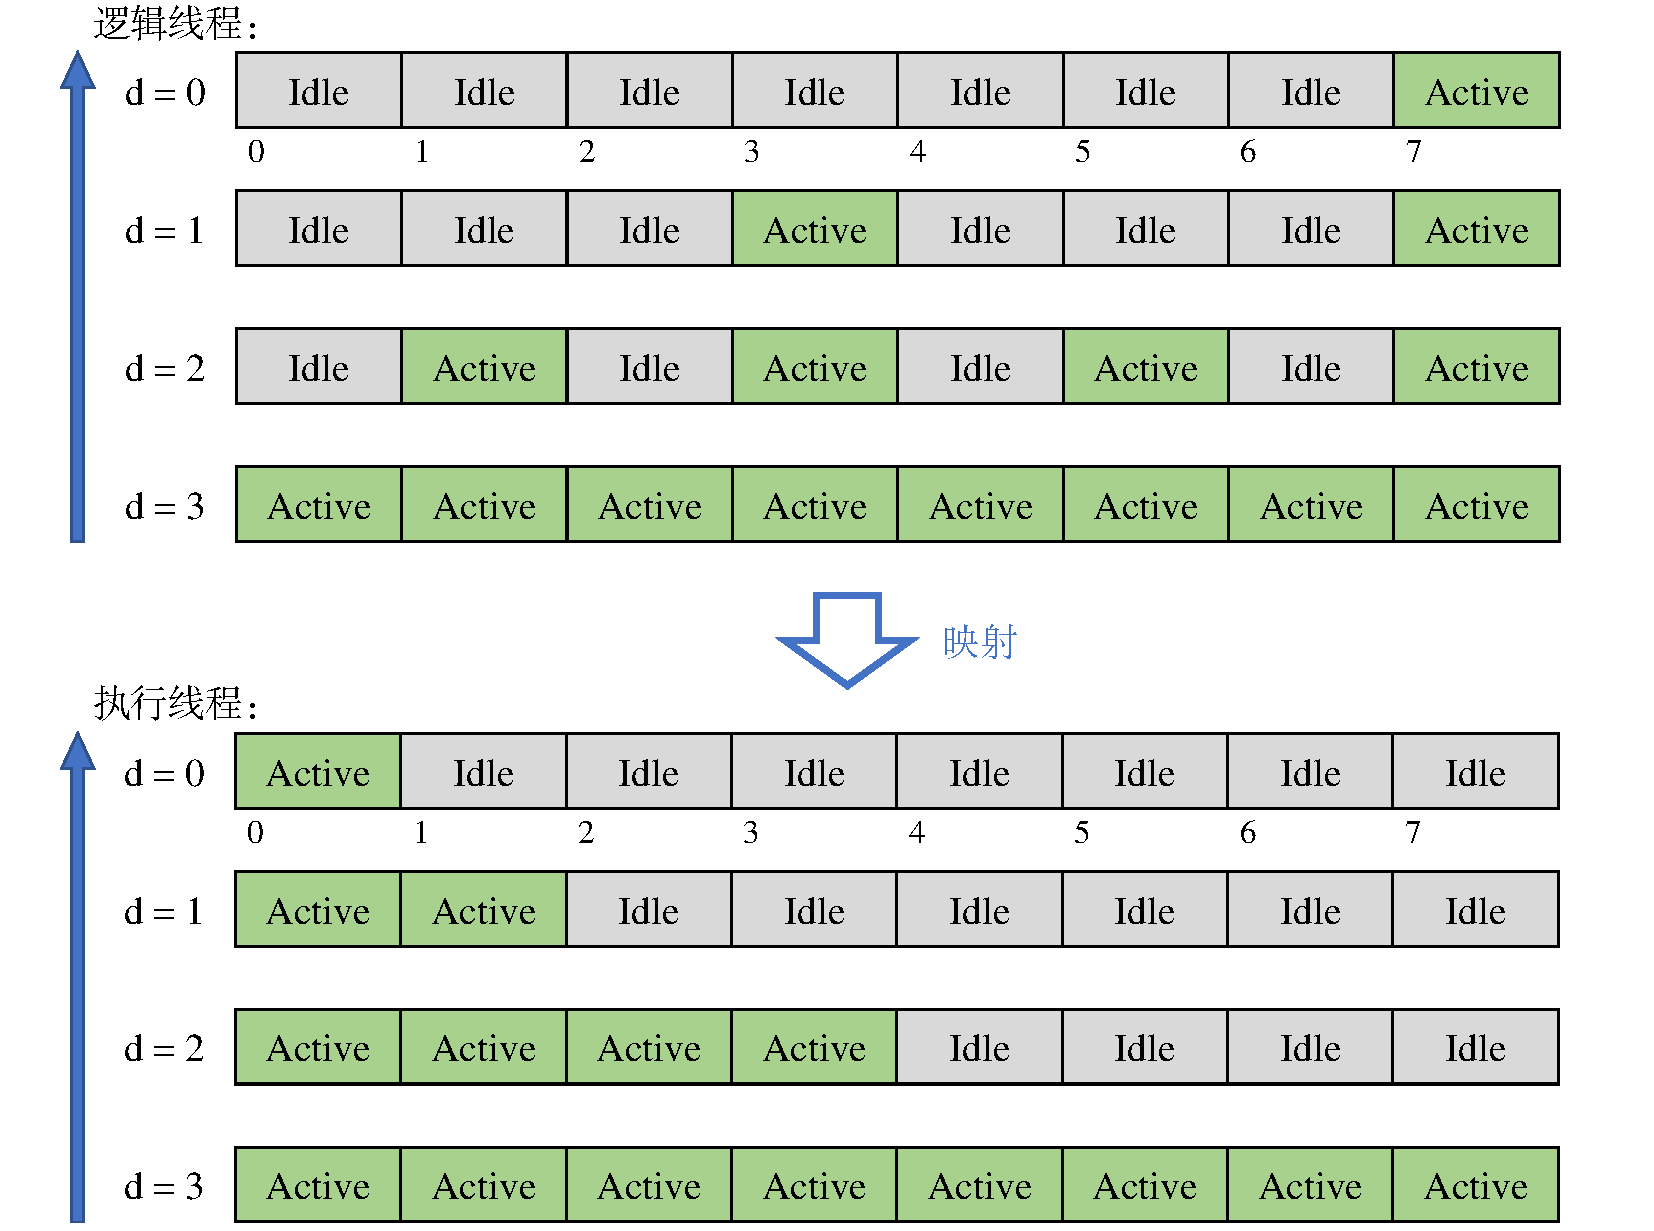
\includegraphics[width=.9\textwidth]{figures/neighbor/branch_divergence.pdf}
    	\caption{线程分支重映射}
    	\label{fig:remap}
    \end{figure}

\subsubsection{分支优化}
    GPU中包含大量计算单元,适合大量数据并行执行,但不适合执行分支指令。在英伟达的GPU架构中,一般32个流处理器组成一个warp。如果一个warp中线程执行的分支不同,则这一组线程就需要执行所有分支的指令,最后根据判断分支真假选择正确的结果,这显然会浪费大量计算资源。所以我们需要程序中连续的线程之间分支结果尽量相同,以减少分支分歧。
    
    但是在前缀和计算的向上以及向下扫描过程中,逻辑上的线程分支显然是不连续的(如图\ref{fig:upsweep}与\ref{fig:downsweep}),所以我们需要增加一层线程索引的映射(如图\ref{fig:remap}),从而使实际执行的线程分歧是连续的。
    
    \begin{figure}
    	\centering
    	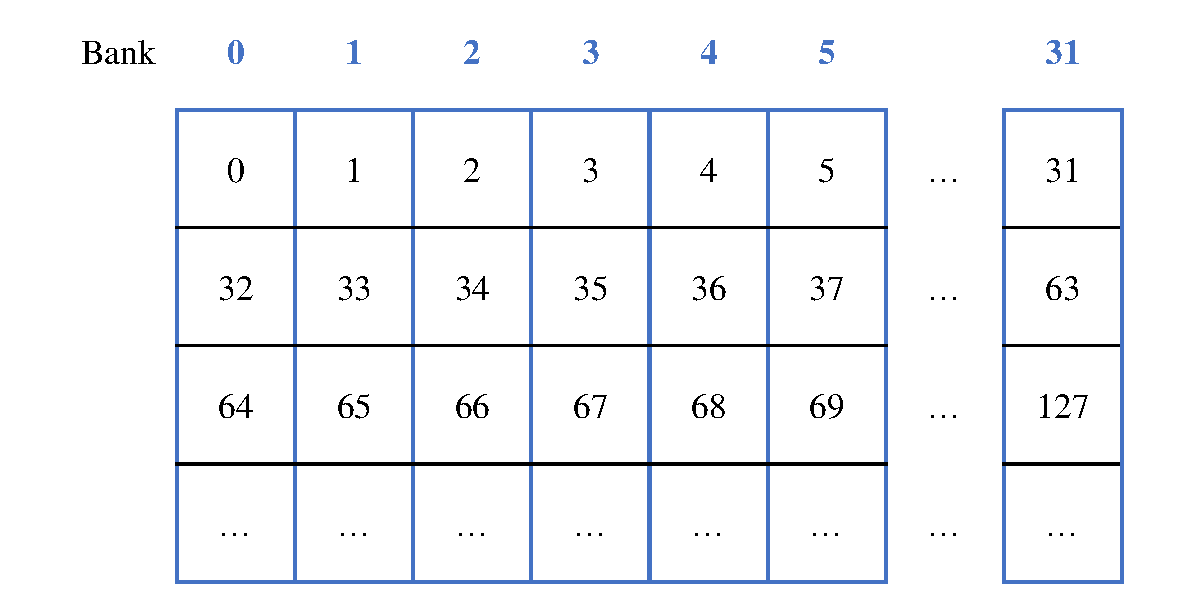
\includegraphics[width=.65\textwidth]{figures/neighbor/bank_conflict.pdf}
    	\caption{共享内存Bank}
    	\label{fig:bank}
    \end{figure}

\subsubsection{避免Bank冲突}
    为了实现共享内存高带宽的并行访问,共享内存被划分成了32个可以同时访问的等大小内存块(Banks,如图\ref{fig:bank}),且每4个字节被分配到了一个Bank中,每个Bank在一个时钟周期的带宽也为4字节。所以在读取共享内存时,如果访问不同Bank中的数据,则不会造成冲突;如果访问同一Bank中的同一个数据,则由于GPU的广播机制,也不会造成冲突;如果访问同一Bank中的不同数据,则由于带宽不足,会发生访存冲突(Bank Conflict),造成线程之间互相等待,使得并行计算退化为串行。
    
    在前缀和计算过程中,每次线程并行执行时访存地址间隔为2的指数倍,会造成Bank冲突。解决方法也很直接,在每32个数据间插入数量不等的空位,打乱访存地址,从而避免Bank冲突。
    
    \begin{figure}
    	\centering
    	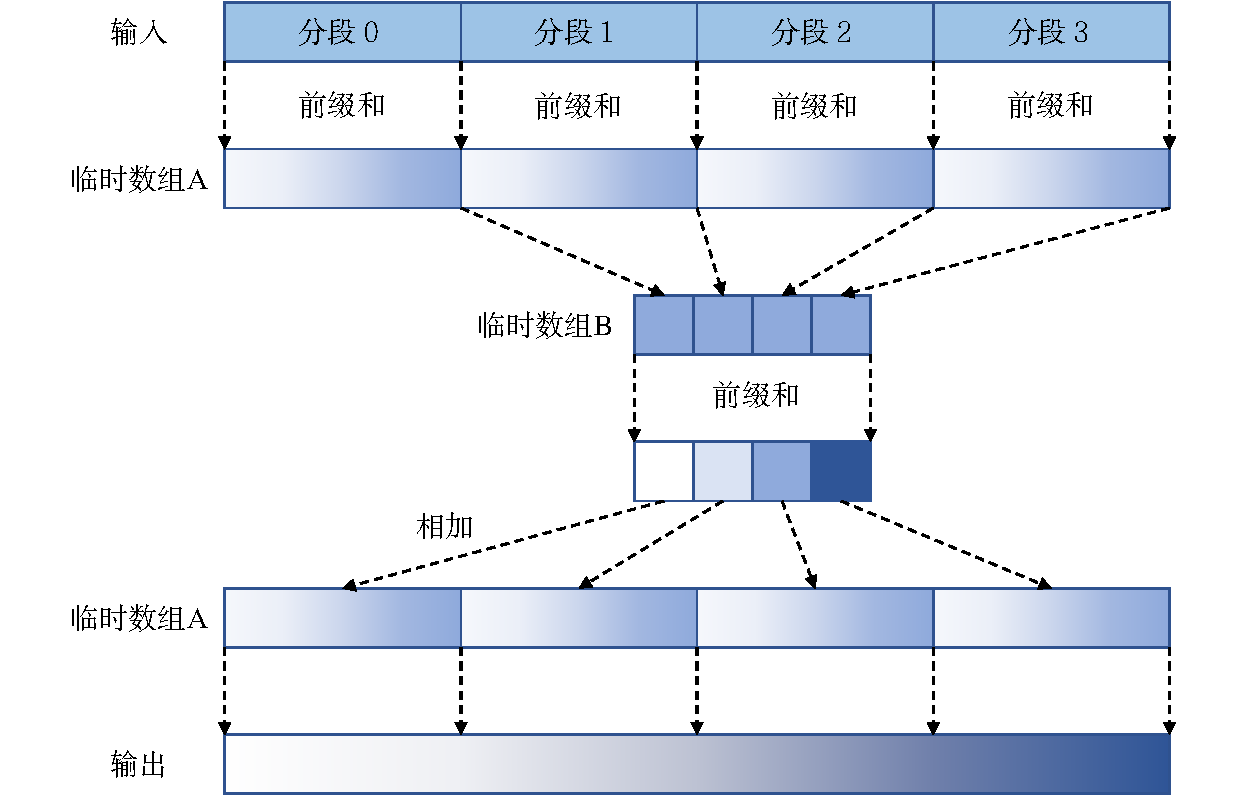
\includegraphics[width=.7\textwidth]{figures/neighbor/big_size_scan.pdf}
    	\caption{递归计算大数组前缀和}
    	\label{fig:bigarryscan}
    \end{figure}

\subsubsection{大数组前缀和}
    前文介绍的数组前缀和计算方法,都建立在同一个线程组的前提下,这是因为共享内存和线程同步指令都只能作用于相同的线程组。而由于WebGPU的限制,同一线程组最高支持256个线程(CUDA中最高支持1024个线程),这意味着我们只能计算最大长度位512的数组前缀和(每个线程读取两个数组元素),这显然是不够的。我们可以使用“递归”的思想解决这个问题(如图\ref{fig:bigarryscan}),对大数组以512长度分段,分别在每段内计算前缀和,再提取每段最后一个元素构成新数组,计算其前缀和,最后将结果加回对应段内的每一个元素。经过一次“递归”后,我们前缀和算法支持的数组最大长度为 $512\times512=2^{18}$(256k)。因此,我们的流体仿真系统最高支持将空间划分为256k个网格,同理,最大流体粒子数量也为256k。


\subsection{本章小结}
    本章详细阐述了邻域粒子并行搜索算法。其主要思想是空间在划分均匀网格来加速搜索,无论是寻找网格粒子,还是构建邻域粒子集,都使用了集合数组这一数据结构。在存储方式上,本章采用了不定长格式的存储结构,降低了存储消耗且增强了算法空间局部性。在其构建方法上,本章使用了计数排序的算法。另外,本章详细介绍了如何数组前缀和算法,他是实现计算排序的核心。尽管这一算法在逻辑上简单明了,但是由于其计算时数据间相互存在依赖,所以使用GPU高效并行化并不容易。最后,本章结合GPU硬件架构(如图\ref{fig:turing}),分别给出了在访存、分支与Bank冲突三方面的算法优化方案。